\documentclass[handout, 10pt]{beamer}

%\usepackage[backend=bibtex,firstinits=true,style=verbose-inote,citestyle=authortitle]{biblatex}
\usepackage{bm}
\usepackage{graphicx}
\usepackage{subcaption}
\usepackage{amsmath}
\usepackage{amsfonts}
\usepackage{makecell}
\usepackage{filecontents}
\usepackage{biblatex}
\usepackage{xcolor}
\usepackage{subcaption}
 \newcommand{\expect}[2][]{
\ifthenelse{\equal{#1}{}}{
\mathbb{E}\left[#2\right]
}{
\underset{#1}{\mathbb{E}}\left[#2\right]
}}

\newcommand{\cov}[2][]{
\ifthenelse{\equal{#1}{}}{
\text{Cov}\left[#2\right]
}{
\underset{#1}{\text{Cov}}\left[#2\right]
}}


\newcommand{\var}[2][]{
\ifthenelse{\equal{#1}{}}{
\text{Var}[#2]
}{
\underset{#1}{\text{Var}}[#2]
}}

\newcommand{\loss}[2][]{
\ifthenelse{\equal{#1}{}}{
\mathcal{L}(#2)
}{
\mathcal{L}_{#1}(#2)
}}

\newcommand{\kl}[2]{
\text{D}_\text{KL}[#1 \parallel #2]
}

\newcommand{\R}{\mathbb{R}}
%\newcommand{\Prob}{\mathbb{P}}

\newcommand{\1}[1]{\mathds{1}\{#1\}}


%\usecolortheme{dolphin}
\setbeamertemplate{navigation symbols}{}
\setbeamertemplate{section in toc}{\inserttocsectionnumber.~\inserttocsection}

\begin{filecontents*}{references.bib}
@inproceedings{gan_rewriting,
 title={Rewriting a Deep Generative Model},
 author={Bau, David and Liu, Steven, and Wang, Tongzhou, and Zhu,
 Jun-Yan and Torralba, Antonio},
 booktitle={Proceedings of the European Conference on Computer Vision (ECCV)},
 year={2020}
}
\end{filecontents*}

\addbibresource{references.bib}


\title{Rewriting a Deep Generative Model\footnote{\citepaper{gan_rewriting}}}
%\subtitle{}
%\author{Ivan Skorokhodov}
%\date{}
%\logo{
\includegraphics[height=1cm]{images/ipavlov-logo.png}}

\newcommand{\citepaper}[1]{\citetitle{#1} by \citeauthor{#1}, \citeyear{#1}}

%\graphicspath{{./images}}

%\usetheme{lucid}
\begin{document}

\begin{frame}
    \titlepage
\end{frame}

\begin{frame}{Overview}
\begin{itemize}
    \item\pause \textit{Rewriting a generator} means changing its weights in such a way that it now generates a different distribution
\begin{figure}
\centering
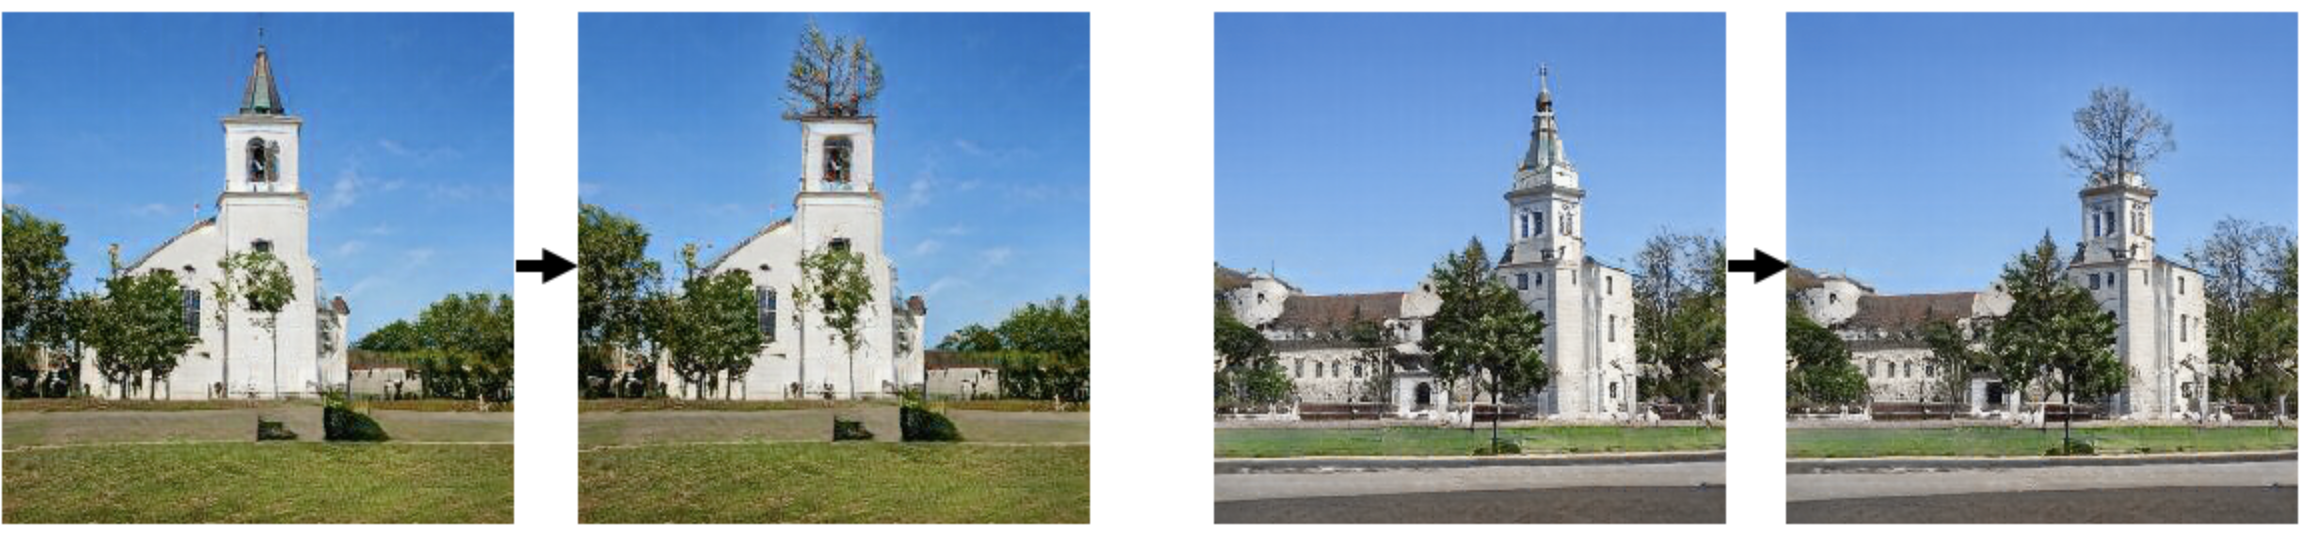
\includegraphics[width=\textwidth]{images/rewriting-churches}
\caption{An example of rewriting: generator now generates churches with trees on top of their domes}
\end{figure}
    \item\pause Authors provide a different perspective on NN layers as key-value memory banks
    \item\pause They rewrite G by inserting a new key-value pair into one of its layers
\end{itemize}
\end{frame}


\begin{frame}{An old way to do rewriting}
\begin{itemize}
    \item\pause Imagine that we want to rewrite $G(z, \theta_0)$
    \item\pause For this, we first generate several $x_i = G(z_i, \theta_0)$ for different $z_i$
    \item\pause Then we update each $x_i \mapsto x_{*i}$ to describe our new rule
    \begin{itemize}
        \item\pause For example, photoshop a hat on a horse' head
        \begin{figure}
            \centering
            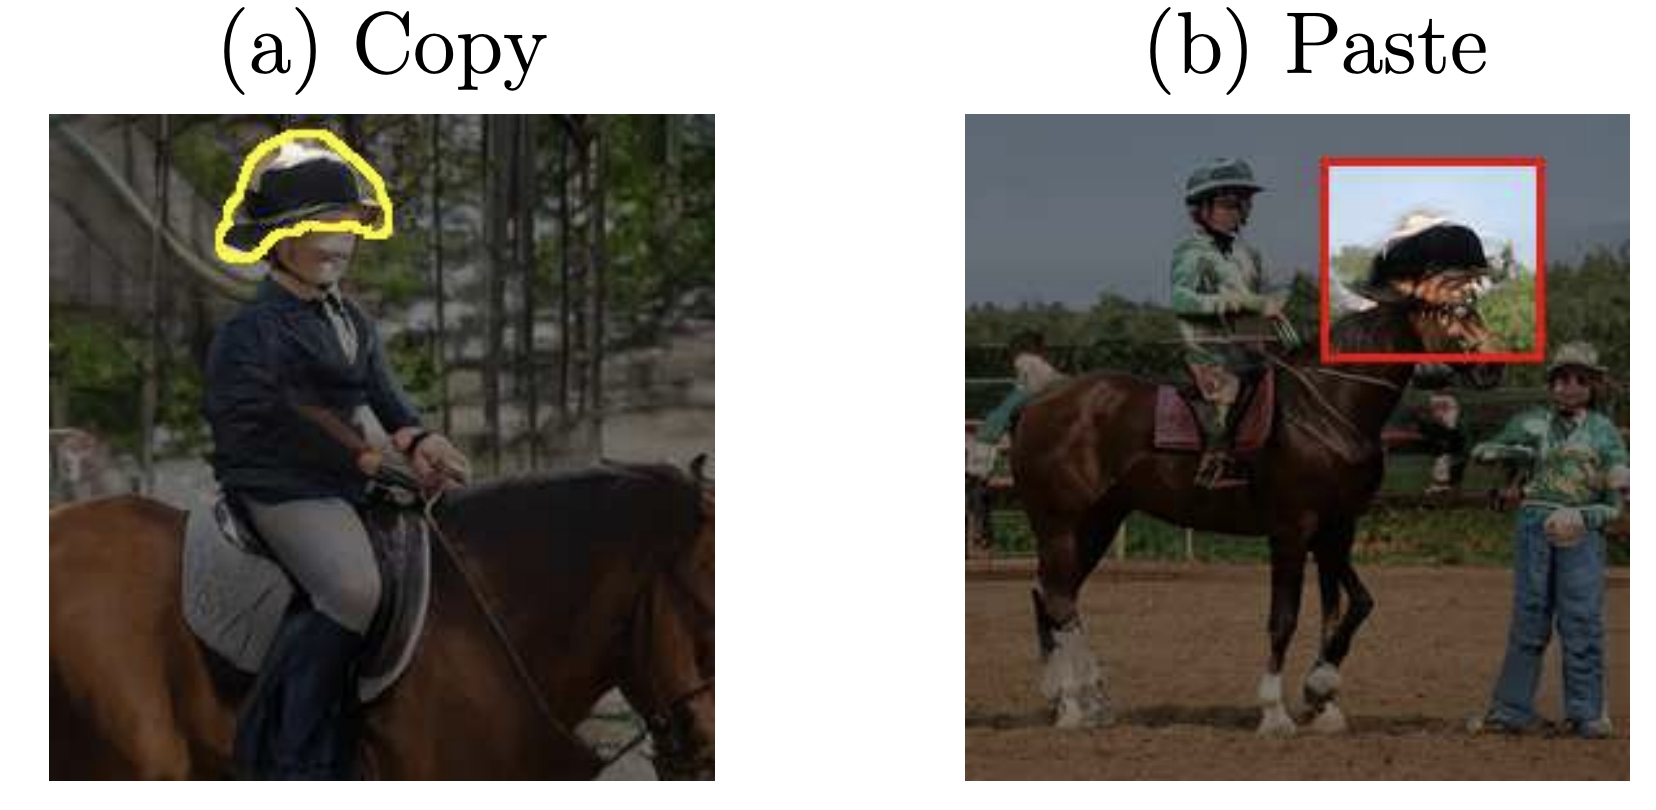
\includegraphics[width=0.7\textwidth]{images/horse-hat-photoshop}
        \end{figure}
    \end{itemize}
\end{itemize}
\end{frame}


\begin{frame}{An old way to do rewriting (continued)}
\pause
Now, find the ``rewrited'' $G$ parameters $\theta_1$ by minimizing:
    \begin{equation}
\begin{aligned}
\theta_{1} =\arg \min _{\theta} \mathcal{L}_{\text {smooth }}(\theta)+\lambda \mathcal{L}_{\text {constraint }}(\theta)
\end{aligned}
\end{equation}

\pause
$\mathcal{L}_{\text {smooth }}$ helps us not to deviate from old images:
    \begin{equation}
        \mathcal{L}_{\text {smooth }}(\theta) \triangleq \mathbb{E}_{z}\left[\ell\left(G\left(z ; \theta_{0}\right), G(z ; \theta)\right)\right]
    \end{equation}
    
\pause
$\mathcal{L}_{\text {constraint }}$ helps us to enforce the rule:
    \begin{equation}
        \mathcal{L}_{\text {constraint }}(\theta) \triangleq \sum_{i} \ell\left(x_{* i}, G\left(z_{i} ; \theta\right)\right)
    \end{equation}

\pause
Unfortunately, $G$ overfits and does not generalize too well

\pause
But authors found that this strategy works much better if we optimize over a single layer instead of all the parameters
\end{frame}


\begin{frame}{NN layers are memory banks}
\begin{itemize}
    \item\pause We can see a linear layer $y = Wx$ as an associative memory (a 50-year old idea):
\begin{equation}
    v_i \approx W k_i
\end{equation}
    \item\pause So, instead of input-output pairs we now have key-value pairs
    \item\pause I.e., given an input $k_i$, layer $W$ ``recalls'' output $v_i$.
    \item\pause From this perspective, rewriting can be seen as overwriting key $k_i$ with new value $v_{*i}$ (or inserting a new one)
    \item\pause For a convolutional layer, we just convert $n_\text{in} \times k \times k \times n_\text{out}$ tensor into $(n_\text{in} \cdot k \cdot k) \times (n_\text{out})$ matrix
\end{itemize}
\end{frame}


\begin{frame}{Rewriting by memory update in a linear case}
\begin{itemize}
    \item\pause We now can rewrite $G$ by overwriting one of its keys $k_*$ in layer $W^\ell$
    \item\pause For this, we solve the optimization problem:
    \begin{equation}
\begin{aligned}
W_{1} &=\underset{W}{\arg \min }\|V-W K\|^{2} \qquad\text { s.t. } v_{*} =W_{1} k_{*}
\end{aligned}
\end{equation}
    \item\pause It has an analytical solution, but authors develop a different perspective to be able to generalize to non-linear transforms
\end{itemize}
\end{frame}


\begin{frame}{Rewriting by memory update in a \textit{non}-linear case}
\begin{itemize}
    \item\pause NN layers are usually non-linear transforms: $y = f(x, W)$
    \item\pause This still can be seen as an associative memory $v_i = f(k_i, W)$
    \item\pause In this case, there is no analytical solution to update the memory
    \item\pause But for a linear case, we can shown that
\begin{equation}
W_{1}=W_{0}+\Lambda\left(C^{-1} k_{*}\right)^{\top}
\end{equation}
where
\begin{equation}
\Lambda_{1}=\underset{\Lambda \in \mathbb{R}^{M}}{\arg \min }\left\|v_{*}- [W_{0}+\Lambda (C^{-1} k_{*})^\top] k_*\right\|
\end{equation}
\item\pause Authors generalize this procedure to a non-linear case by finding $\Lambda_1$ via:
\begin{equation}
\Lambda_{1}=\underset{\Lambda \in \mathbb{R}^{M}}{\arg \min }\left\|v_{*}-f\left(k_{*} ; W_{0}+\Lambda (C^{-1} k_{*})^\top\right)\right\|
\end{equation}
\end{itemize}
\end{frame}


\begin{frame}{Rewriting procedure visualization}
\begin{figure}
\centering
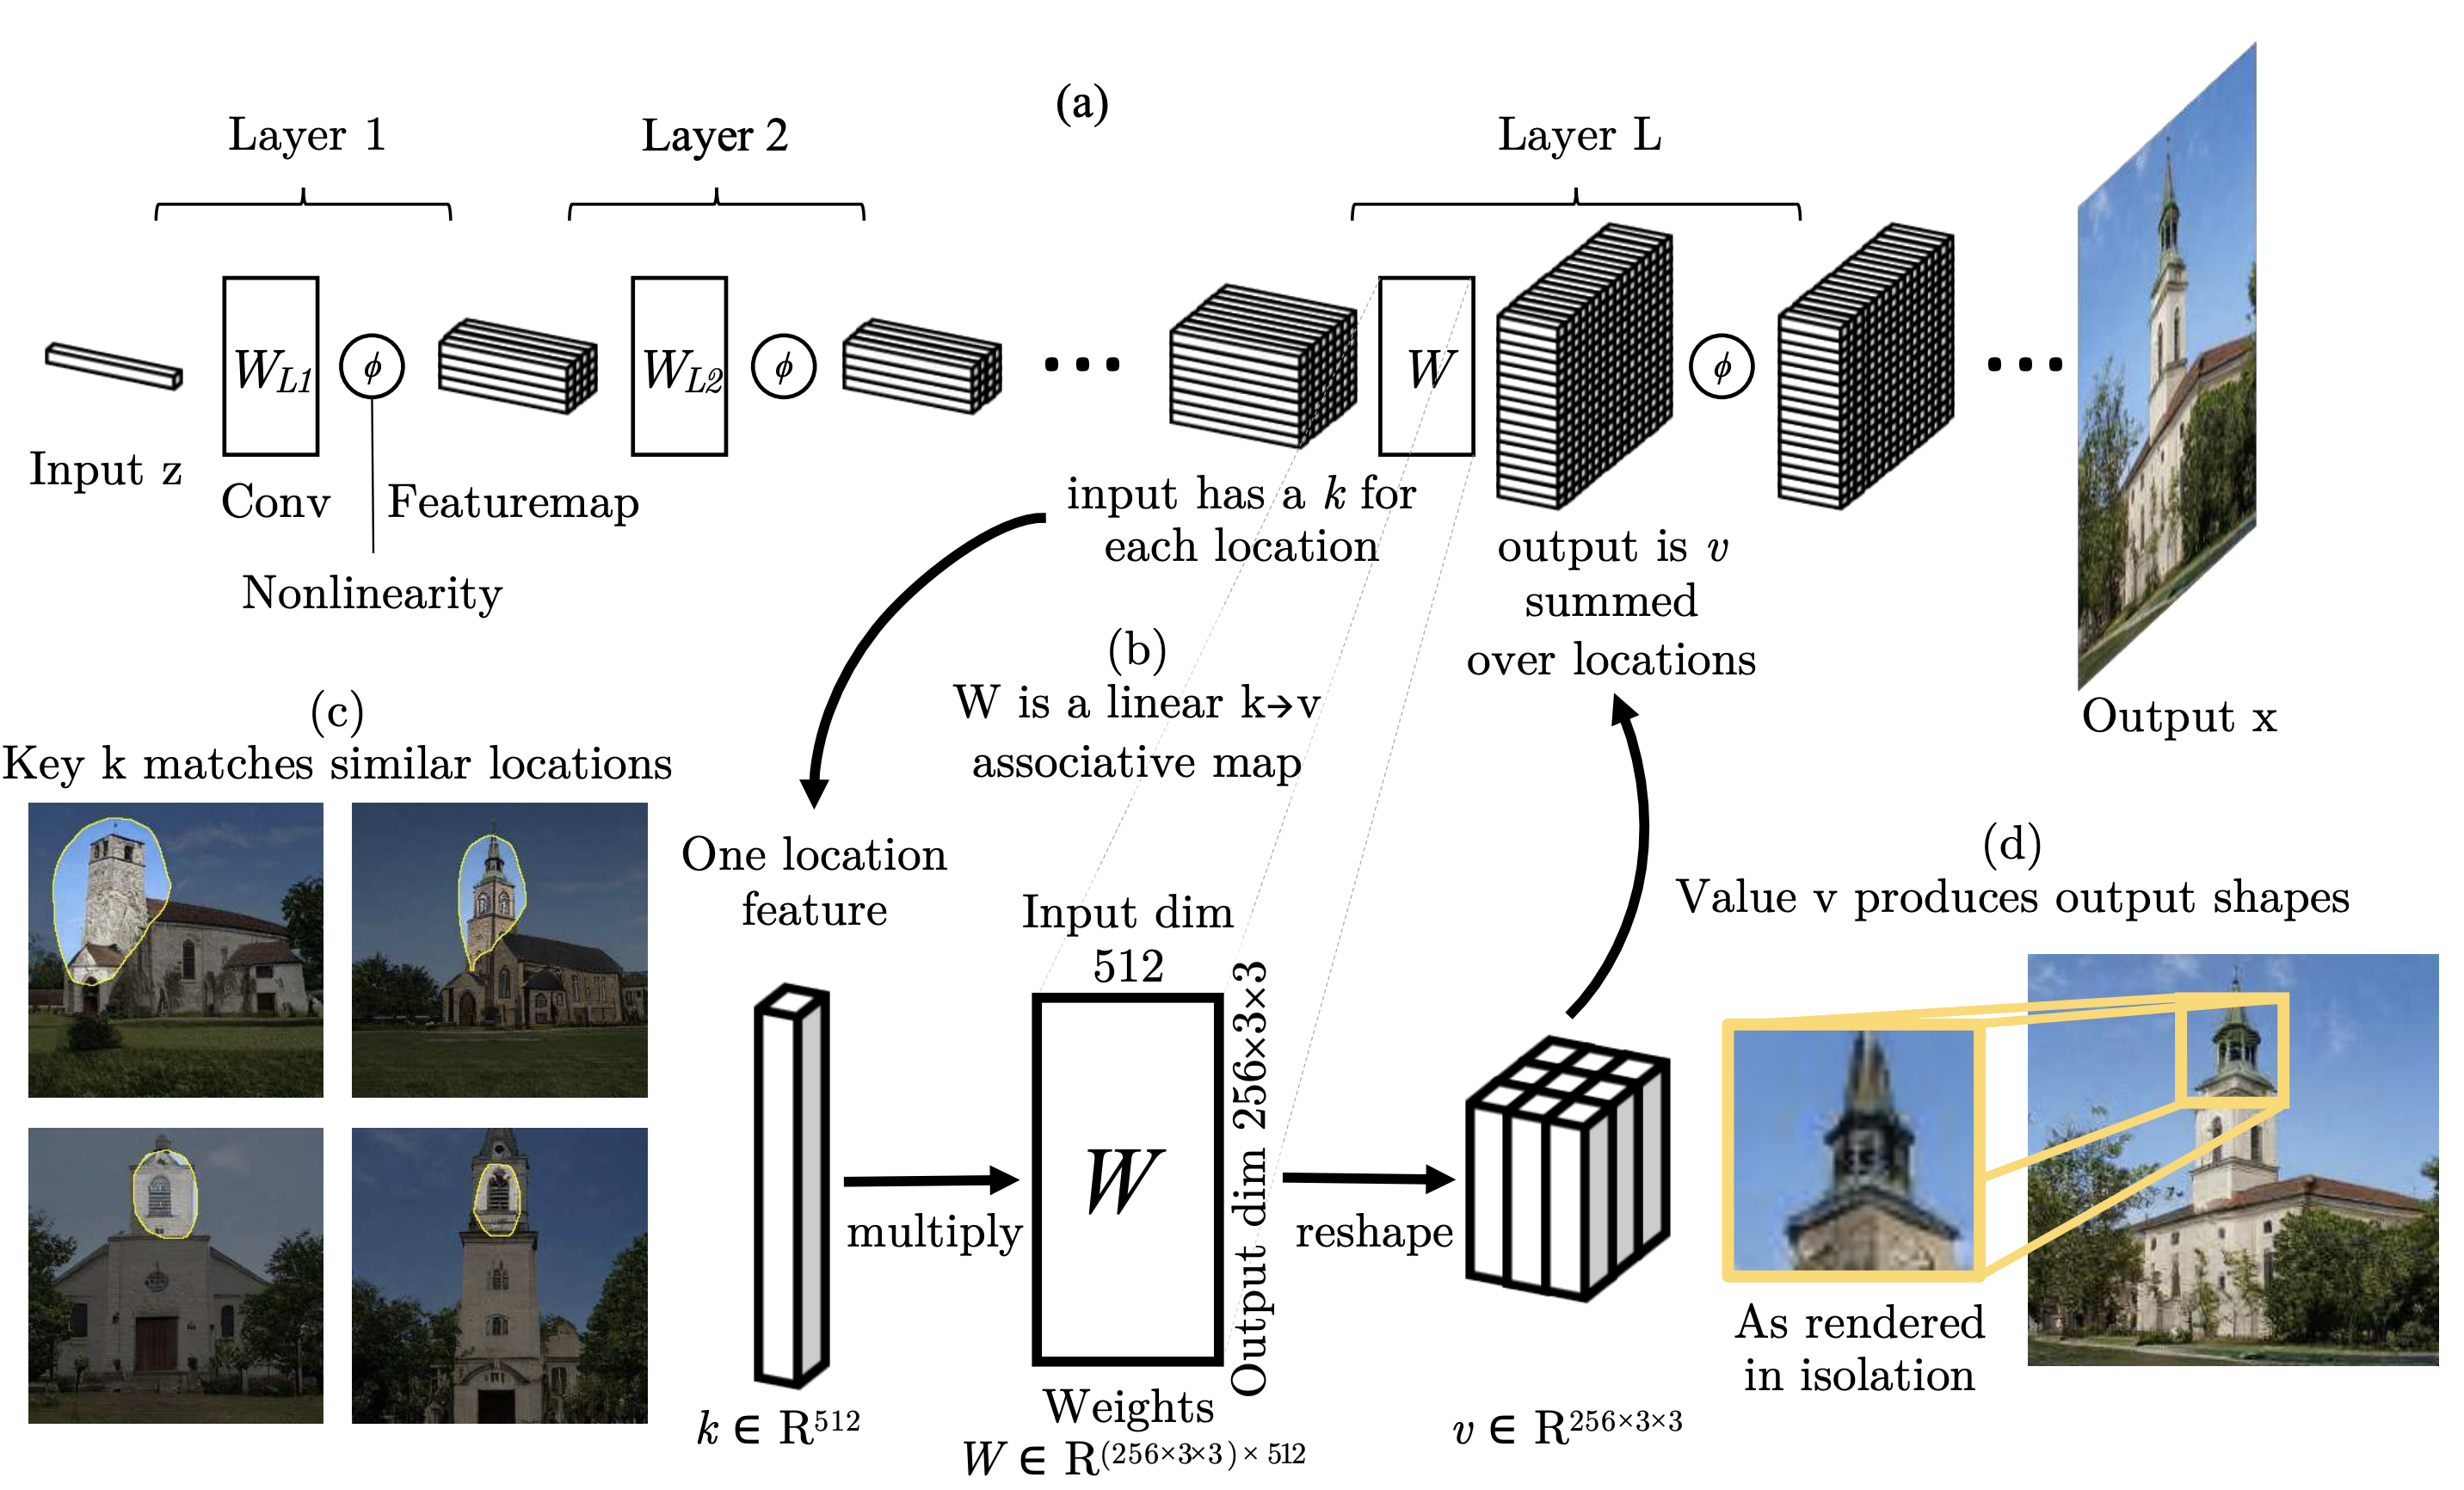
\includegraphics[width=\textwidth]{images/rewriting-visualization.png}
\end{figure}
\end{frame}


\begin{frame}{Qualitative results}
\begin{figure}
\centering
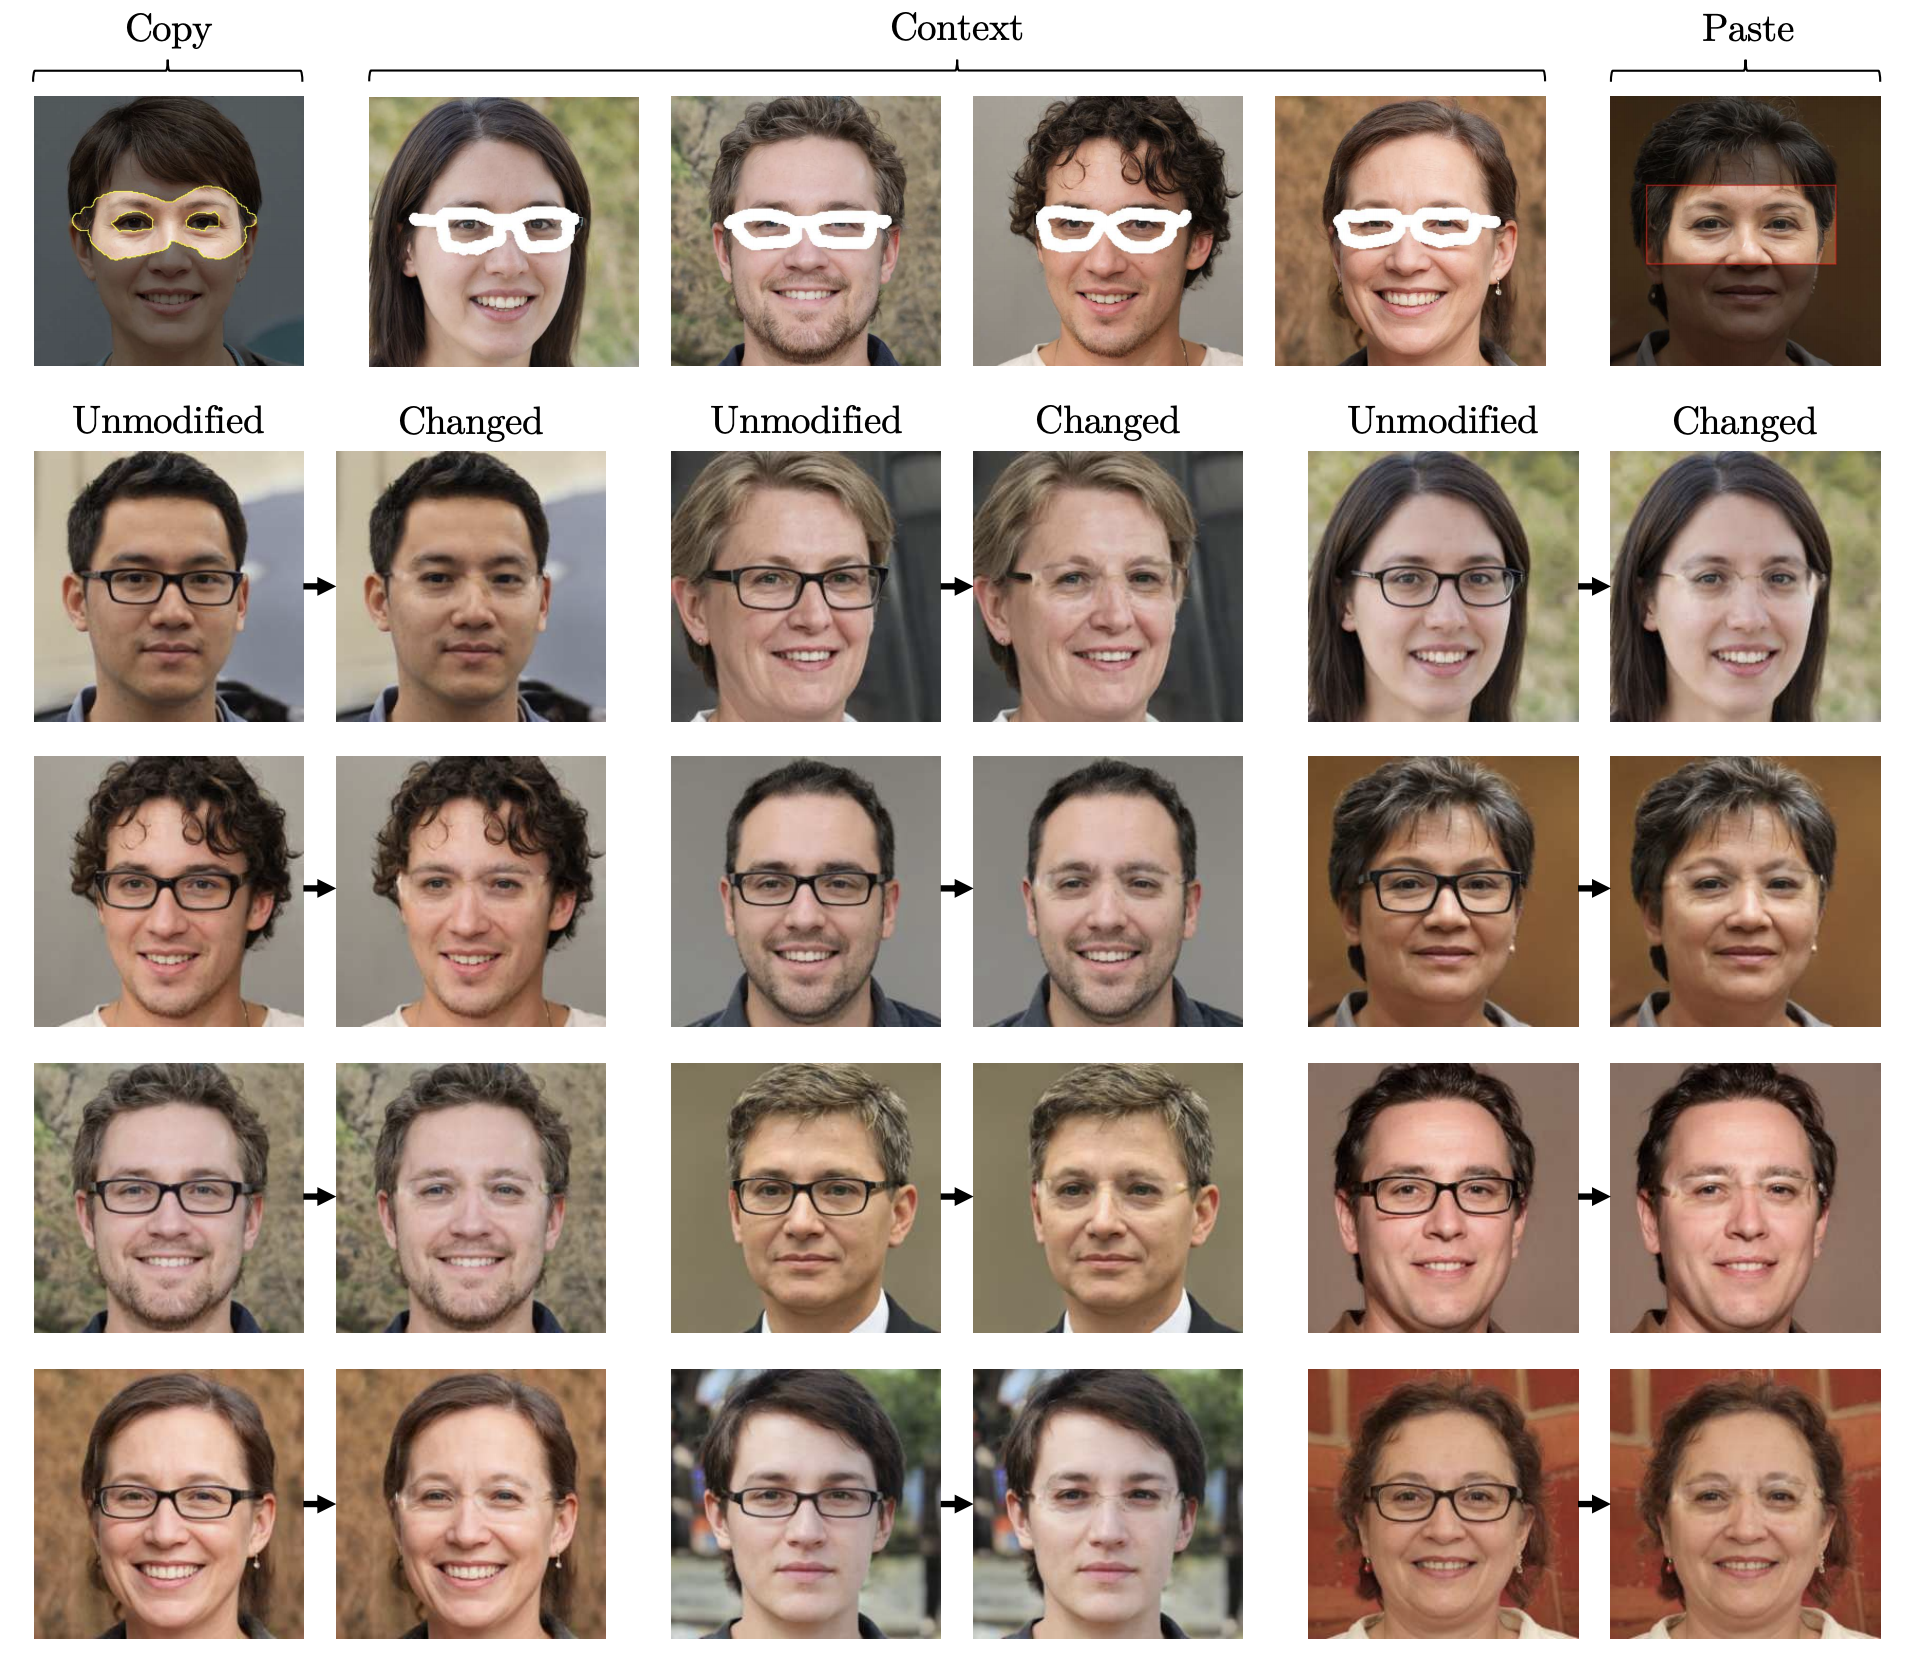
\includegraphics[width=0.8\textwidth]{images/removing-eyeglasses}
\end{figure}
\end{frame}


\begin{frame}{Final thoughts}
\begin{itemize}
    \item Rewriting shows a powerful property of modern GANs
    \item But generator does not know how to blend a new value nicely with the novel context
    \begin{itemize}
        \item That's why for many samples results look clumsily ``copy-pasted''
        \item How can we alleviate this?
        \item (Results still look impressive)
    \end{itemize}
    \item Associative memory perspective is very interesting since this is how human memory works
\end{itemize}
\end{frame}


\end{document}
